% course:       CV
% teacher:      DongHui Wang
% author:       zju_cs / Yi Zhang / 21721190
% mail:         yizhangzc@gmail.com
% data:         2018/5
% environment:  ubuntu 16.04 / texlive-full / texlive-xetex      
% compiler:     xelatex / bibtex

\documentclass[a4paper]{article}

\usepackage{ctex}           % support chinese
\usepackage{geometry}       % setting margin
\usepackage{setspace}       % setting space
\usepackage{graphicx}       % support insert iamge
\usepackage{subcaption}


\title{Classification@affNIST dataset}
\date{2018-05}
\author{张毅\hspace{1em}21721190}

\geometry{left=3cm,right=3cm,top=2.5cm,bottom=2.5cm}

\begin{document}

    \pagenumbering{gobble}
    
    \begin{center}
        \doublespacing
        
        \Large \textbf{Classiffication@affNIST dataset}

        \normalsize 姓名:张毅 \qquad 学号:21721190 \qquad 日期:2018-5
    \end{center}

    \section{问题描述}

    在AffNIST数据集上训练模型进行分类任务,识别0-9十个数字。

    数据集: AffNIST(https://www.cs.toronto.edu/~tijmen/affNIST/),训练数据与测试数据默认已经划分好,试验中采用默认的划分方式。

    \section{方法及原理}

    实验中采用了比较常用的KNN和SVM对图片进行分类,代码已经上传到github仓库(yizhangzc/course),本次实验与第二次实验代码均放置在classification文件夹下,运行方式及运行环境见README.md。
    
    KNN:如果一个样本在特征空间中的k个最相邻的样本中的大多数属于某一个类别,则该样本也属于这个类别,并具有这个类别上样本的特性。

    SVM:基于结构风险最小化理论之上在特征空间中构建最优超平面,使得学习器得到全局最优化。对于线性不可分的情况,通过使用非线性映射算法将低维输入空间线性不可分的样本转化为高维特征空间使其线性可分。

    \section{实验结果}

    试验直接在原始数据上进行,每个训练样本作为1600维的向量输入模型进行训练。由于数据集太大,训练时间非常长,所以分别只使用了训练与测试集中的部分样本(每个.mat文件中均取1000个样本)。最终结果为:

        \begin{center}
            KNN:\qquad 准确率:68.8\% \qquad f1值:67.5\%

            SVM:\qquad 准确率:82.2\% \qquad f1值:82.0\%
        \end{center}

        \begin{figure}[htbp]
            \centering
            \begin{subfigure}[b]{0.4\textwidth}
                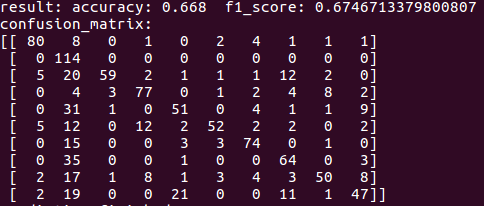
\includegraphics[width=\textwidth]{./images/confusion_matrix_knn.png}
                \caption{KNN混淆矩阵}
            \end{subfigure}
            \begin{subfigure}[b]{0.4\textwidth}
                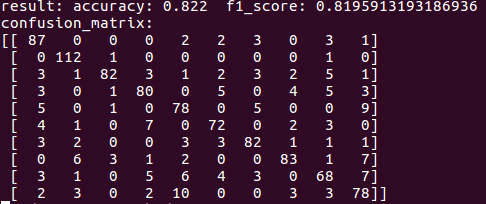
\includegraphics[width=\textwidth]{./images/confusion_matrix_svm.png}
                \caption{SVM混淆矩阵}
            \end{subfigure}
            
            \label{fig:confusion_matrix}
        \end{figure}

    \section{总结}

    (1)实验在1600维的向量上进行,未能成功尝试先提取特征在使用KNN或SVM进行分类比较遗憾。(2)SVM调参至关重要,使用sklearn包中的默认参数效果极差(大约20\%),通过实验,得到效果比较好的参数是,kernel:高斯,gamma:0.03,C:30。(3)KNN中K对模型的影响相对较小,最终取值5。

\end{document}